\documentclass[12pt]{article}

\usepackage{wrapfig}
\usepackage[spanish]{babel}
\usepackage[utf8]{inputenc}
\usepackage{amsmath}
\usepackage{graphicx}
\usepackage[colorinlistoftodos]{todonotes}

\begin{document}

\begin{titlepage}

\newcommand{\HRule}{\rule{\linewidth}{0.5mm}} % Defines a new command for the horizontal lines, change thickness here

\center % Center everything on the page
 
%----------------------------------------------------------------------------------------
%	HEADING SECTIONS
%----------------------------------------------------------------------------------------

\textsc{\LARGE Universidad de Sonora} \\ [0.4cm]

\includegraphics[scale=.65]{./Images/Logo} \\ [0.3cm]
\textsc{\LARGE Física computacional I}\\[0.3cm]

%----------------------------------------------------------------------------------------
%	TITLE SECTION
%----------------------------------------------------------------------------------------

\HRule \\

{\huge \bfseries Actividad 3\\
Análisis de datos con Pandas y visualización con Plotly\\}

 \HRule \\ [1cm]
\vfill

\begin{minipage}{0.6\textwidth}
	\raggedright
	\large
	\textbf{Gómez García, Manuel Ignacio}
\end{minipage}
~
\begin{minipage}{0.35\textwidth}
	\raggedleft
	\large
	\textbf{9/Diciembre/2018}
\end{minipage}

\end{titlepage}

\section{Introducción}

\noindent La presente práctica se enfoca en realizar un análisis de datos de las mareas, salinidad y temperatura registrada por los diversos sensores colocados alrededor del manglar conocido como \textit{El sargento}. Los datos recopilados constan de la presión atmosférica, nivel del mar, temperatura, salinidad y conductividad, así como la fecha y hora correspondiente de cada medición. \\
\indent Tras analizar los datos proporcionados podremos determinar si existe alguna correlación entre las variables y de qué tipo es, pero antes debemos conocer un poco más acerca de la marea y la salinidad del agua. \\
\indent La marea, la cual es originada por la atracción gravitacional que ejercen el Sol y la Luna sobre nuestros mares, en conjunto con la erróneamente llamada "fuerza centrífuga", resultante del movimiento angular de la Tierra. Como mencionamos, es principalmente la Luna quien afecta más nuestros mares debido a que se encuentra mucho más cerca del planeta, por lo tanto, la posición en la que se encuentre es de gran importancia pues de ello dependen las mareas bajas (bajamar) y las mareas altas (pleamar), tan así de importante es que durante el día se generan dos mareas de cada tipo cada 12 horas. \\
\indent La salinidad del mar, como bien dice el mismo nombre, hace referencia a la cantidad de sal disuelta en un litro de agua de mar, sin embargo, es posible que dicho valor sea variante en ciertas áreas debido a la evaporación, estancamiento o flujo de agua con distinta salinidad. Es importante conocer este valor pues tiene repercusiones en el entorno que la contiene, como en su flora y fauna.

\section{Desarrollo}

\noindent Para llevar a cabo el análisis de los datos crearemos un par de gráficas que correspondan con las variables que nos interesan pero antes de ello debemos procesar los datos que nos fueron proporcionados directamente desde la estación en el manglar con el fin de asegurar que sean los necesarios.

\subsection{Importación de bibliotecas}

\noindent Comenzamos importando al cuadernilllo de trabajo las bibliotecas que serán necesarias (figura \ref{fig:importacion}).

\begin{figure}[h!]
	\raggedright
	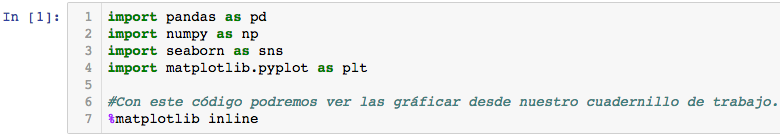
\includegraphics[scale=.6]{./Images/importacion}
	\caption{\label{fig:importacion} Bibliotecas empleadas en el código.}
\end{figure}

\subsection{Lectura de archivos}

\noindent Después procedemos a leer los archivos .CSV de cada estación del manglar (figura \ref{fig:lectura}).

\begin{figure}[h!]
	\center
	%\raggedright
	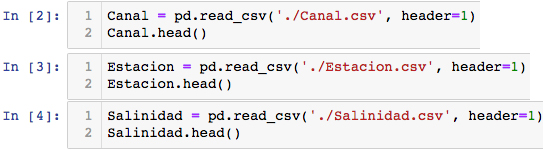
\includegraphics[scale=.6]{./Images/lectura}
	\caption{\label{fig:lectura} Configuración utilizada para la lectura.}
\end{figure}

\subsection{Preparación de los datos}

\noindent Al momento de leer los archivos .CSV los datos no siempre tienen un formato muy claro o, en ocasiones, presentan ciertos inconvenientes como celdas vacías, información irrelevante, columnas o filas con errores, etcétera. Por eso mismo deben ser procesados previo a trabajar con ellos.

\subsubsection{Eliminar datos innecesarios}

\noindent En esta ocasión, los datos contenían una columna llamada '\textit{\#}', la cual enumeraba cada registro hecho en la base de datos pero ahora no es necesario, así que eliminaremos esta columna (figura \ref{fig:eliminar}).

\begin{figure}[h!]
	\center
	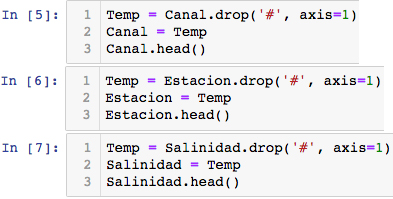
\includegraphics[scale=.6]{./Images/eliminar}
	\caption{\label{fig:eliminar} Removemos la columna '\textit{\#}' de cada archivo.}
\end{figure}

\subsubsection{Cambio de formato}

\noindent Entre nuestros datos tenemos una columna para la fecha y hora llamada '\textit{Fecha}', sin embargo, el formato que presenta es \textbf{object} (se percibe como texto) cuando lo más conveniente es que sea \textbf{datetime} para tener un manejo de la información mucho más sencillo (figura \ref{fig:formato}).

\begin{figure}[h!]
	\center
	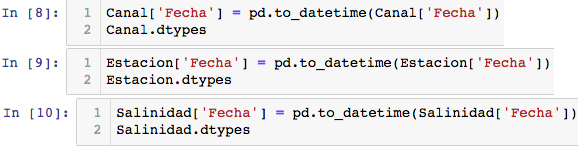
\includegraphics[scale=.6]{./Images/formato}
	\caption{\label{fig:formato} Modificamos el tipo de la columna '\textit{Fecha}' a datetime.}
\end{figure}

\subsubsection{Renombrar columnas}

\noindent Modificaremos los encabezados de cada columna, de modo que presenten nombres más cortos, comprensibles y sin caracteres que puedan ocasionar problema al leerlos (figura \ref{fig:renombrar}).

\begin{figure}[h!]
	\center
	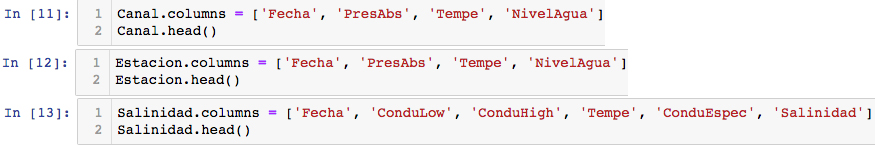
\includegraphics[scale=.55]{./Images/renombrar}
	\caption{\label{fig:renombrar} Renombramos las columnas para evitar errores posteriormente.}
\end{figure}

\subsection{Creación de gráficas}

\noindent En este punto, la información ya tiene un orden apropiado con el cual podremos crear algunas gráficas para buscar una correlación entre los diversos factores analizados. Haremos esto para períodos de tiempo de un día y una semana). \\
\indent Entre las gráficas a crear tenemos:

\begin{itemize}
	\item[-] Nivel del mar en la estación y del canal.
	\item[-] Salinidad y nivel del mar junto a la estación.
    \item[-] Temperatura del agua en la estación y el canal.
    \item[-] Correlación entre el nivel de agua y la salinidad.
\end{itemize}

\subsubsection{Datos por períodos}

\noindent Como mencionamos anteriormente haremos dos nuevos arreglos para trabajar, uno de ellos con un período de un día; el otro, una semana. Para hacer esto tendremos que delimitar el rango de fechas con el cual trabajaremos mediante un par de variables (figura \ref{fig:limites}).

\begin{figure}[h!]
	\center
	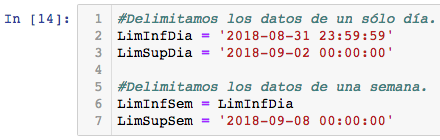
\includegraphics[scale=.6]{./Images/limites}
	\caption{\label{fig:limites} Limites para los períodos de tiempo.}
\end{figure}

Una vez hecho esto, lo siguiente es crear nuevos marcos de información con los limites establecidos y además asegurarnos que tengan la misma cantidad de información (filas) pues de no ser así puede ocasionar dificultades (figura \ref{fig:diasem}).

\begin{figure}
	\center
	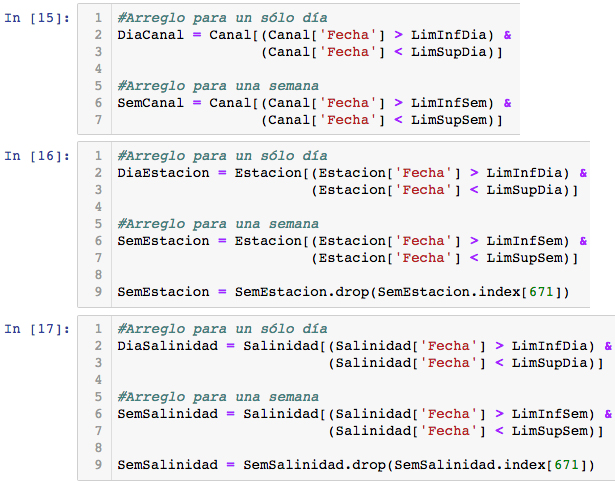
\includegraphics[scale=.6]{./Images/diasem}
	\caption{\label{fig:diasem} Creación de nuevos marcos de información y delimitados.}
\end{figure}

\subsubsection{Gráficas}

\noindent Finalmente es posible proceder a crear las gráficas mencionadas en un principio.\\
\\ 
%-----------------------------------------------------------------------------------------------------------------------
\textbf{Nivel del mar} \\
Está gráfica muestra el comportamiento del nivel del mar en la estación y el canal del manglar durante un día y una semana. \\
\\
• Código empleado para un día (figura \ref{fig:code-nivel-dia}).

\begin{figure}[h!]
	\raggedright
	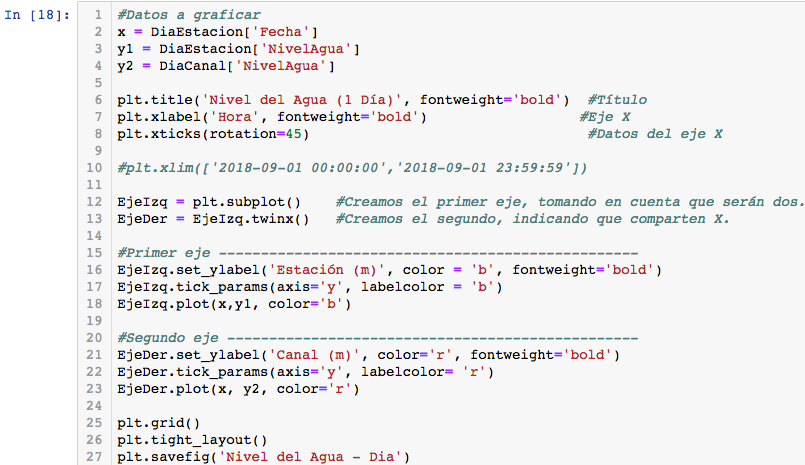
\includegraphics[scale=.6]{./Images/nivel-dia}
	\caption{\label{fig:code-nivel-dia} Configuración para generar la gráfica del nivel del mar de un día.}		
\end{figure}

\noindent • Gráfico generado para un día (figura \ref{fig:graf-nivel-dia}).

\begin{figure}[h!]
	\center
	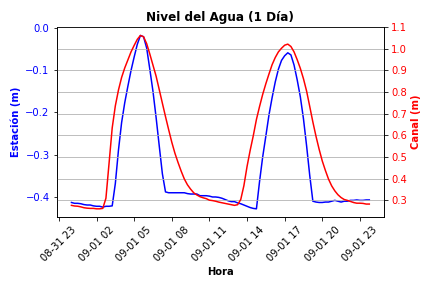
\includegraphics[scale=.6]{Nivel-del-Agua-Dia}
	\caption{\label{fig:graf-nivel-dia} Gráfica resultante para el nivel del mar durante un día.}
\end{figure}

\noindent • Código empleado para una semana (figura \ref{fig:code-nivel-sem}).

\begin{figure}[h!]
	\raggedright
	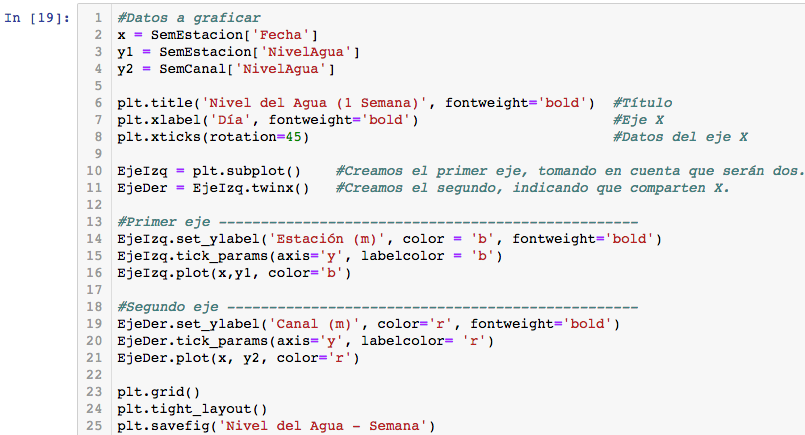
\includegraphics[scale=.6]{./Images/nivel-sem}
	\caption{\label{fig:code-nivel-sem} Configuración para generar la gráfica del nivel del mar de una semana.}		
\end{figure}

\noindent • Gráfico generado para una semana (figura \ref{fig:graf-nivel-sem}).

\begin{figure}[h!]
	\center
	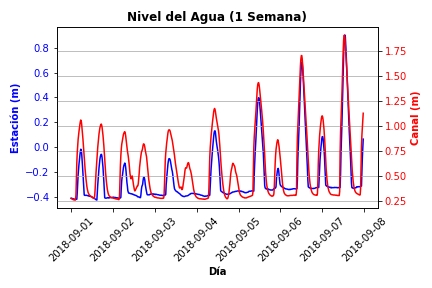
\includegraphics[scale=.6]{Nivel-del-Agua-Semana}
	\caption{\label{fig:graf-nivel-sem} Gráfica resultante para el nivel del mar durante una semana.}
\end{figure}
%-----------------------------------------------------------------------------------------------------------------------

\pagebreak

%-----------------------------------------------------------------------------------------------------------------------
\noindent \textbf{Salinidad y nivel del mar} \\
La gráfica muestra el comportamiento de la salinidad y el nivel del agua en la estación del manglar durante un día y una semana. \\
\\
• Código empleado para un día (figura \ref{fig:cod-sal-dia}). \\

\begin{figure}[h!]
	\center
	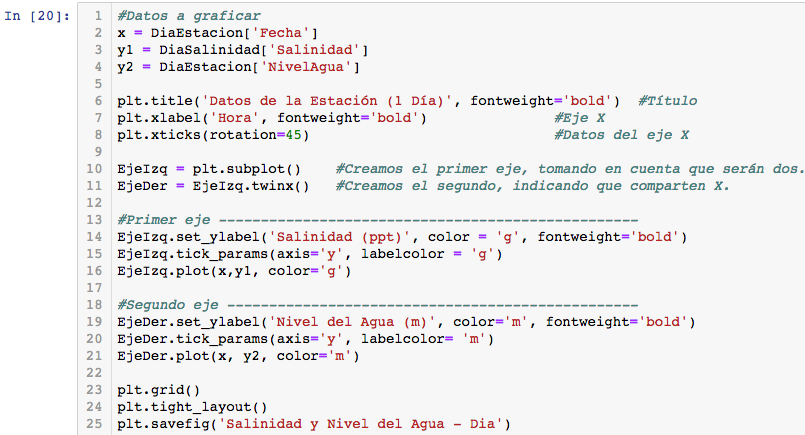
\includegraphics[scale=.6]{./Images/sal-dia}
	\caption{\label{fig:cod-sal-dia} Configuración para generar la gráfica de salinidad y nivel del mar de un día.}
\end{figure}

\noindent • Gráfico generado para un día (figura \ref{fig:graf-sal-dia}). \\

\begin{figure}[h!]
	\center
	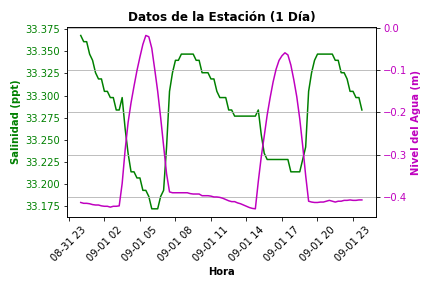
\includegraphics[scale=.6]{Salinidad-y-Nivel-del-Agua-Dia}
	\caption{\label{fig:graf-sal-dia} Gráfica resultante de la salinidad y nivel del mar durante un día.}
\end{figure}

\noindent • Código empleado para una semana (figura \ref{fig:cod-sal-sem}). \\

\begin{figure}[h!]
	\center	
	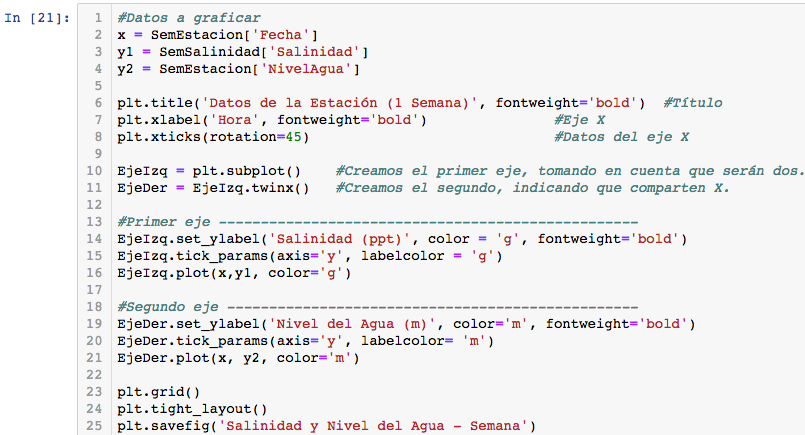
\includegraphics[scale=.6]{./Images/sal-sem}
	\caption{\label{fig:cod-sal-sem} Configuración para generar la gráfica de salinidad contra nivel del mar por una semana.}
\end{figure}

\noindent • Gráfico generado para una semana (figura \ref{fig:graf-sal-sem}). \\

\begin{figure}[h!]
	\center
	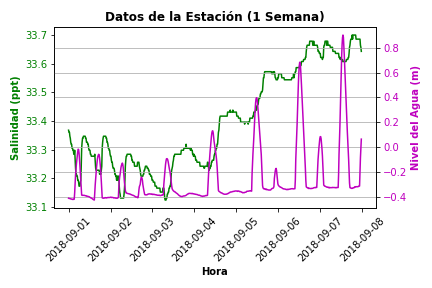
\includegraphics[scale=.6]{Salinidad-y-Nivel-del-Agua-Semana}
	\caption{\label{fig:graf-sal-sem} Gráfica resultante de la salinidad y el nivel del mar durante una semana.}
\end{figure}
%-----------------------------------------------------------------------------------------------------------------------
\noindent \textbf{Temperatura del agua} \\
La gráfica muestra el comportamiento de la temperatura del agua en la estación y el canal del manglar durante un día y una semana. \\
\\
• Código empleado para un día (figura \ref{fig:cod-temp-dia}). \\

\begin{figure}[h!]
	\center
	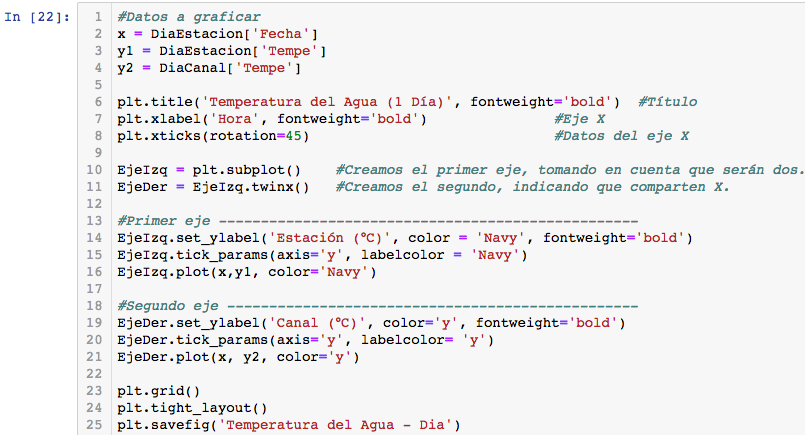
\includegraphics[scale=.6]{./Images/temp-dia}
	\caption{\label{fig:cod-temp-dia} Configuración para generar la gráfica de la temperatura del mar en la estación y el canal del manglar por un día.}
\end{figure}

\noindent • Gráfico generado para un día (figura \ref{fig:graf-temp-dia}). \\

\begin{figure}[h!]
	\center
	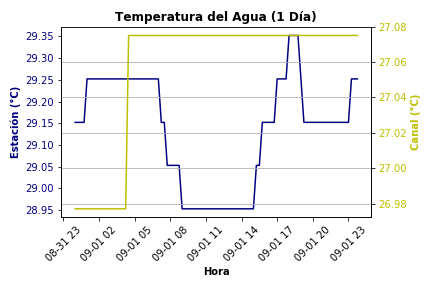
\includegraphics[scale=.6]{Temperatura-del-Agua-Dia}
	\caption{\label{fig:graf-temp-dia} Gráfica resultante para la temperatura del mar durante un día.}
\end{figure}

\noindent • Código empleado para una semana (figura \ref{fig:cod-temp-sem}). \\

\begin{figure}[h!]
	\center
	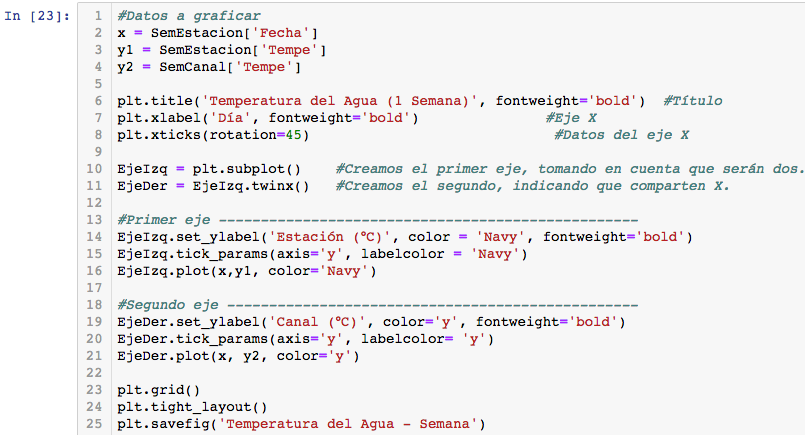
\includegraphics[scale=.6]{./Images/temp-sem}
	\caption{\label{fig:cod-temp-sem} Configuración para generar una gráfica de temperatura del mar de la estación y el canal del manglar durante una semana.}
\end{figure}

\noindent • Gráfico generado para una semana (figura \ref{fig:graf-temp-sem}). \\

\begin{figure}[h!]
	\center
	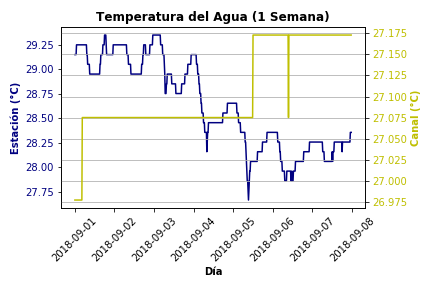
\includegraphics[scale=.6]{Temperatura-del-Agua-Semana}
	\caption{\label{fig:graf-temp-sem} Gráfico correspondiente a la temperatura del mar en la estación y canal del manglar durante una semana.}
\end{figure}
%-----------------------------------------------------------------------------------------------------------------------
\noindent \textbf{Correlación} \\
La siguiente tabla mostrará la correlación entre cada una de las variables con el resto de ellas. \\

\noindent • Código empleado para un día (figura \ref{fig:cod-corre-dia}). \\

\begin{figure}[h!]
	\center
	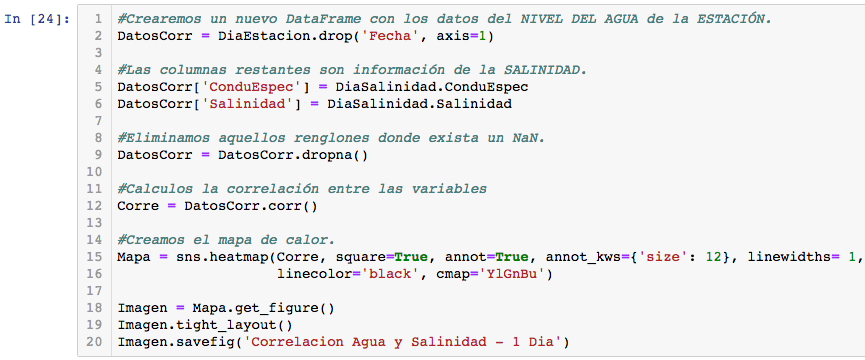
\includegraphics[scale=.55]{./Images/corre-dia}
	\caption{\label{fig:cod-corre-dia} Configuración para la tabla de correlación por un día.}
\end{figure}

\noindent • Gráfico generado para un día (figura \ref{fig:graf-corre-dia}). \\

\begin{figure}[h!]
	\center
	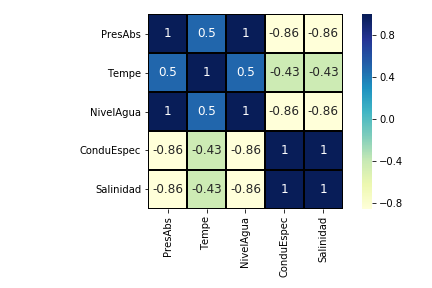
\includegraphics[scale=.6]{Correlacion-Agua-y-Salinidad-Dia}
	\caption{\label{fig:graf-corre-dia} Tabla generada mostrando la correlación entre las variables durante un día.}
\end{figure}

\noindent • Código empleado para una semana (figura \ref{fig:cod-corre-sem}). \\

\begin{figure}[h!]
	\center
	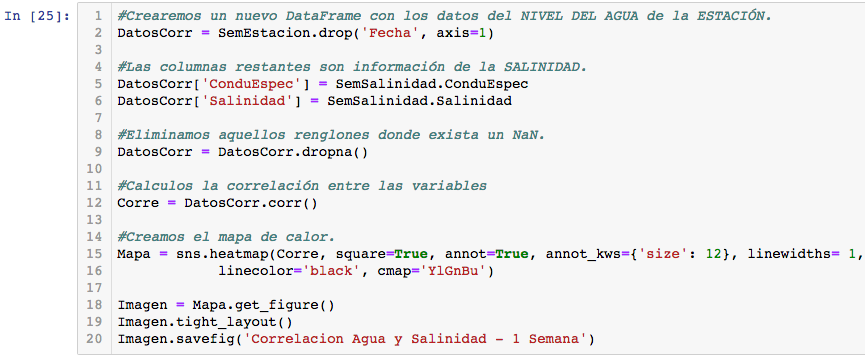
\includegraphics[scale=.55]{./Images/corre-sem}
	\caption{\label{fig:cod-corre-sem} Configuración para la tabla de correlación por una semana.}
\end{figure}

\noindent • Gráfico generado para una semana (figura \ref{fig:graf-corre-sem}).

\begin{figure}[h!]
	\center
	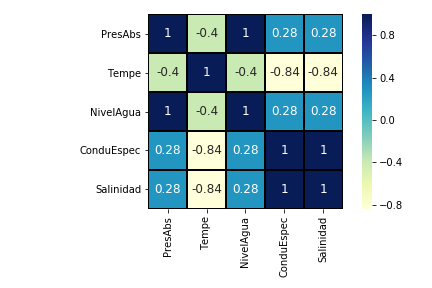
\includegraphics[scale=.6]{Correlacion-Agua-y-Salinidad-Semana}
	\caption{\label{fig:graf-corre-sem} Tabla generada mostrando la correlación entre las variables durante una semana.}
\end{figure}

\subsection{Nuevos datos}

\noindent Agregamos unos cuantos datos más para tener una vista más amplía de estos y ver posibles ciclos a lo largo de los meses, y para hacer esto haremos nuevamente cada unos de los pasos iniciales más uno extra para agregar todo.

\subsubsection{Procesamiento de los datos}

\noindent Los pasos realizados para estos nuevos datos serán los mostrados en la figura \ref{fig:procesamiento}.

\begin{figure}[h!]
	\center
	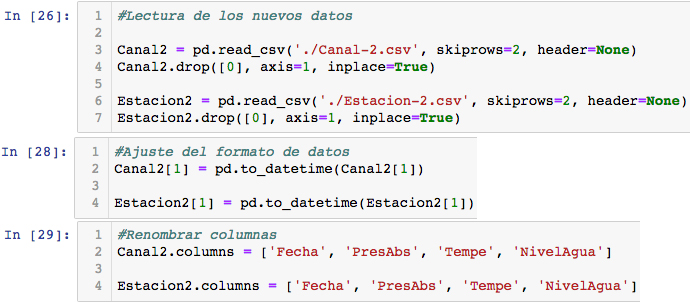
\includegraphics[scale=.6]{./Images/procesamiento}
	\caption{\label{fig:procesamiento} Tratamiento entero para los nuevos datos.}
\end{figure}

\subsubsection{Adición de datos}

\noindent Para proceder en este punto debemos agregar los datos originales y los nuevos en un sólo marco de datos (figura \ref{fig:suma}).

\begin{figure}[h!]
	\center
	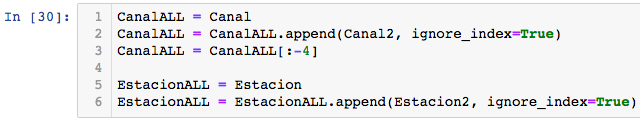
\includegraphics[scale=.6]{./Images/sumadf}
	\caption{\label{fig:suma} Código empleado para la limpieza de los datos.}
\end{figure}

\subsubsection{Gráfico resultante}

\noindent La siguiente gráfica muestra el nivel del mar en la estación y el canal a lo largo de aproximadamente 2 meses. \\

\noindent • Código empleado para la configuración del gráfico (figura \ref{fig:cod-nivel-total}). \\

\begin{figure}[h!]
	\center
	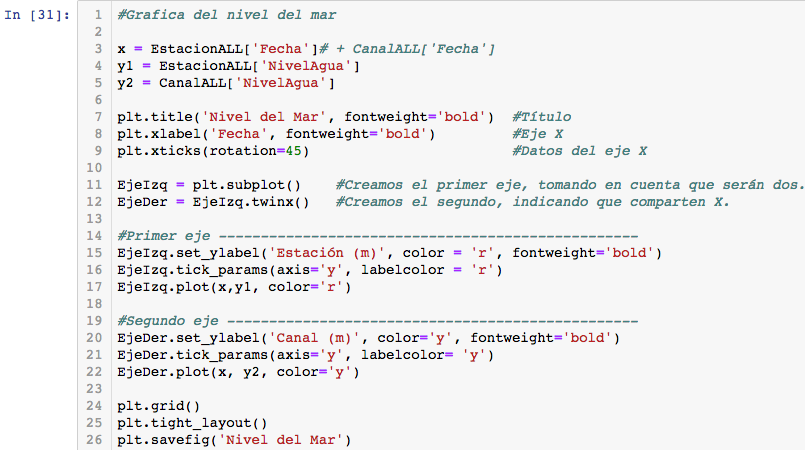
\includegraphics[scale=.6]{./Images/nivel-doble}
	\caption{\label{fig:cod-nivel-total} Código empleado para la gráfica del nivel del mar con todos los datos.}
\end{figure}

\noindent • Gráfica generada para el nivel del mar (figura \ref{fig:graf-nivel-total}).

\begin{figure}[h!]
	\center
	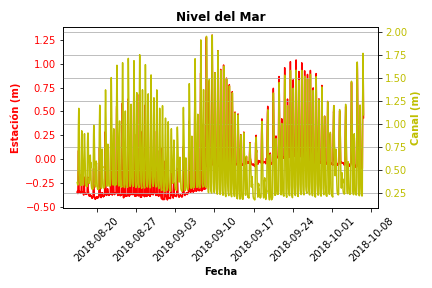
\includegraphics[scale=.6]{Nivel-del-Mar}
	\caption{\label{fig:graf-nivel-total} Gráfica del nivel del mar registrados en la estación y canal del manglar del registro total.}
\end{figure}

\section{Conclusión}

\noindent Para dar una conclusión habrá que basarse en los resultados observados en las tabla de correlación de un día y una semana. \\ [0.5em]
\noindent \textbf{Valores de correlación para un día} \\
\indent • Presión atmosférica absoluta y nivel del mar (1) \\
\indent • Conductividad específica y salinidad (1) \\
\indent • Presión atmosférica absoluta y temperatura del mar (0.5) \\
\indent • Temperatura del mar y nivel del mar (0.5) \\
\indent • Temperatura del mar y conductividad específica (-0.43) \\
\indent • Temperatura del mar y salinidad (-0.43) \\
\indent • Presión atmosférica absoluta y conductividad específica (-0.86) \\
\indent • Presión atmosférica absoluta y salinidad (-0.86) \\
\indent • Nivel del mar y conductividad específica (-0.86) \\
\indent • Nivel del mar y salinidad (-0.86) \\

\pagebreak

\noindent \textbf{Valores de correlación para una semana} \\
\indent • Presión atmosférica absoluta y nivel del mar (1) \\
\indent • Conductividad específica y salinidad (1) \\
\indent • Presión atmosférica absoluta y conductividad específica (0.28) \\
\indent • Presión atmosférica absoluta y salinidad (0.28) \\
\indent • Nivel del mar y conductividad específica (0.28) \\
\indent • Nivel del mar y salinidad (0.28) \\ 
\indent • Presión atmosférica absoluta y temperatura del mar (-0.4) \\
\indent • Temperatura del mar y nivel del mar (-0.4) \\
\indent • Temperatura del mar y conductividad específica (-0.84) \\
\indent • Temperatura del mar y salinidad (-0.84) \\

Podemos apreciar que en el período de un día la presión atmosférica absoluta y el nivel del mar, así como la conductividad específica y la salinidad están directamente relacionadas, mientras que la presión atmosférica esta anticorrelacionada con la conductividad específica y salinidad, y de igual manera el nivel del mar con la conductividad específica y salinidad. \\
\indent Durante el período de una semana los resultados arrojados cambiaron pues si bien los valores correlacionados son los mismos, los anticorrelacionados ahora son la temperatura del mar con la conductividad específica y salinidad. \\
\indent Finalmente podemos concluir que la salinidad esta anticorrelacionada con el nivel del mar a corto plazo pero conforme aumentamos el período analizado nos damos cuenta que la salinidad deja de relacionarse tanto con el nivel del mar y más con la temperatura de este.

\begin{thebibliography}{9}
	\bibitem{Mareas} (2016, Noviembre 4). \textsc{La marea, qué es y cómo se forma, mareas vivas y mareas muertas, pleamar y bajamar}. 9 de diciembre del 2018, de Sail and Trip. Recuperado de https://sailandtrip.com/la-marea/
	
	\bibitem{Salinidad} (2013, Octubre 7). \textsc{Salinidad}. 9 de diciembre del 2018, de EcuRed. Recuperado de https://www.ecured.cu/Salinidad

\end{thebibliography}

\end{document}
